\PassOptionsToPackage{dvipsnames}{xcolor}
\documentclass{beamer}
\usepackage{xcolor}
\usepackage{pgfpages}

\usepackage[style=authortitle]{biblatex}

\setbeameroption{show notes on second screen}

\usepackage[utf8]{inputenc}
\usepackage[T1]{fontenc}
\usepackage{lmodern}
\usepackage{fontawesome}

\usepackage{minted}

\usepackage{listings}

\usepackage[american]{babel}

\usepackage{
    amsmath,
    amsfonts,
    amssymb
}

\usepackage[os=win]{menukeys}

\usetheme{UOS}

\graphicspath{{img/}}

% use this with \begin{pythoncode} ... \end{pythoncode}
\newminted{python}{linenos=false}

\newminted[outputcode]{text}{linenos=false}

% this gets rid of red boxes around syntax errors in minted
\AtBeginEnvironment{minted}{%
  \renewcommand{\fcolorbox}[4][]{#4}}

% removes the prefix "Figure 1:" in figure captions
\setbeamertemplate{caption}{\raggedright\insertcaption\par}


\begin{document}

\title[Expyriment]{Week 13: Psychological Experiments with Expyriment}
\subtitle{Basic Programming in Python}

\author[kgross, mpoemsl, sselbach]{Katharina Groß, Martin Pömsl, Sören Selbach}

% change to date of actual lecture
\date{\today}

\begin{frame}[plain]
    \titlepage
\end{frame}


\begin{frame}{Your Vote}
    
    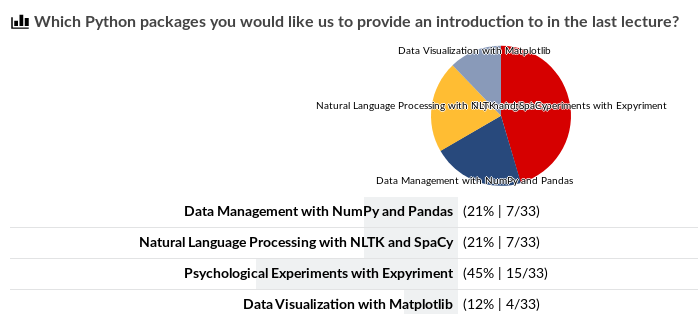
\includegraphics[width=\textwidth]{13_Expyriment/poll.png}
    
\end{frame}

\begin{frame}
    \tableofcontents
\end{frame}


\section{Recap: Using External Packages}


\begin{frame}[fragile]{Installing External Packages}

    \textbf{pip} is the primary package manager of Python. 

    \vspace{1em}

    Most external packages can be installed simply with \texttt{pip install my\_package}.

    \vspace{1em}

    Many packages have dependencies, which means that they build on other packages. \texttt{pip} will usually install all
    dependencies automatically.

    \vspace{1em}

    \textbf{conda} can also be used to install packages with \texttt{conda install my\_package}.

    \note{

        If you have multiple versions of Python on your computer, you should use \texttt{pip3} for Python 3 packages and \texttt{pip2} for Python 2 packages.

        \vspace{1em}

        Official Python guide to module installation:

        \url{https://docs.python.org/3/installing/index.html}

    }

\end{frame}


\begin{frame}[fragile]{Importing External Packages}

    Once they are installed, external packages can be imported just like those from the Standard Library. 

    \vspace{1em}

    If you only require certain submodules of large packages, it is a good idea to selectively import only those with \texttt{from}.

    \vspace{1em}

    For some packages there exist naming conventions because the actual names are too large to be pracitcal. This can be done with \texttt{as}.

    \vspace{1em}

    \begin{pythoncode}
from sklearn import model_selection
import numpy as np
import pandas as pd
    \end{pythoncode}

    \note{

        Official Python guide to module installation:

        \url{https://docs.python.org/3/installing/index.html}

    }

\end{frame}


\section{Graphics in Python}

\begin{frame}[plain]
    \sectionpage
\end{frame}


\begin{frame}[fragile]{Graphical User Interfaces}

    So far we have used the console as a user interface for most of our scripts.

    \vspace{1em}

    This is easy to implement, but is not really user-friendly.

    \vspace{1em}

    If you want to provide a more intuitive user interface, you should consider a \textbf{Graphical User Interface (GUI)}.

    \vspace{1em}

    GUIs also enable more advanced input options such as mouseclicks, drag-and-drop operations, checkboxes, buttons etc. 

    as well as more advanced output options such as displaying images.

    \vspace{1em}

    There are two major packages in Python that provide platform-independent GUIs: \textbf{Tkinter} and \textbf{PyQt}.

    \note{

        Using the console for input and output is mostly practical if you want other programmers to use your script.

        \vspace{1em}

        However, if you want actual users to use your script, it may be better to include a GUI.

        \vspace{1em}

        Tkinter Documentation: 

        \url{https://docs.python.org/3/library/tk.html}

        \vspace{1em}

        PyQt Documentation: 

        \url{https://www.riverbankcomputing.com/static/Docs/PyQt5/}

        
    }

\end{frame}


\begin{frame}[fragile]{PyGame}

    \textbf{PyGame} is a free and open source Python programming language library for making multimedia applications (such as e.g. games).

    \vspace{1em}

    It provides not only a GUI, but also geometric shaps, animations, collisions, audio and many more useful utilities.

    \vspace{1em}

    \centering 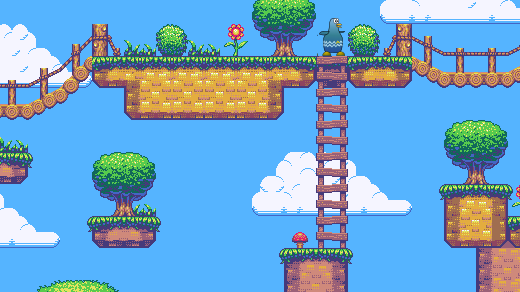
\includegraphics[width=0.6\textwidth]{13_Expyriment/game.png}

    \note{

        This could also be useful for a project!

        \vspace{1em}

        PyGame tutorial: 

        \url{http://openbookproject.net/thinkcs/python/english3e/pygame.html}
        
        \vspace{1em}

        Fun fact: Expyriment is built on top of PyGame!

    }

\end{frame}


\section{Psychological Experiments with Expyriment}

\begin{frame}[plain]
    \sectionpage
\end{frame}


\begin{frame}[fragile]{What is Expyriment?}

    
\includegraphics[width=\textwidth]{13_Expyriment/expyriment.png}

    \textbf{Expyriment} is an open-source and platform independent light-weight Python library for designing and conducting timing-critical behavioural and neuroimaging experiments. 

    \note{

        Documentation:

        \url{https://docs.expyriment.org/}

        \vspace{1em}

        Alternative: PsychoPy

    }

\end{frame}


\begin{frame}[fragile]{Structure}

    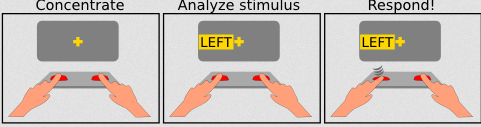
\includegraphics[width=0.9\textwidth]{13_Expyriment/stimulus_response.png}

    \vspace{1em}

    A behavioural experiment in general presents the participants with stimuli and then measures their response to the stimulus.

\end{frame}

\begin{frame}[fragile]{Structure}

    Performing a behavioral experiment is done in two steps:

    \begin{enumerate}

        \item Designing the Experiment: Configuring stimuli and defining the protocol
        \item Executing the Experiment: Executing the protocol and measuring the response 

    \end{enumerate}

    \vspace{1em}

    \begin{pythoncode}
from expyriment import design, control, stimuli, misc
    \end{pythoncode}

    \vspace{1em}

    The submodules \texttt{design} and \texttt{stimuli} are used to design the experiment. \texttt{control} is used to execute the experiment. \texttt{misc} mostly provides useful constants.


\end{frame}


\begin{frame}[fragile]{A Minimal Example}
    \begin{pythoncode}
from expyriment import design, control, stimuli

# Designing the experiment
exp = design.Experiment(name="First Experiment")
control.initialize(exp)
stim = stimuli.TextLine(text="Hello World")
stim.preload()

# Executing the experiment
control.start()
stim.present()
exp.clock.wait(1000)
control.end()
    \end{pythoncode}

\end{frame}

\begin{frame}[fragile]{Designing an Experiment}

    Usually we have more than one stimulus. In order to organize stimuli, there is a strict hierarchy in Expyriment:

    \begin{enumerate}

        \item Blocks: Largest organizing unit. An experiment usually consists of 2-5 blocks.
        \item Trial: Medium organizing unit. A block usually consists of 20-100 trials.
        \item Stimulus: Smallest organizing unit. A single stimulus is e.g. one shape on the screen.

    \end{enumerate}

\end{frame}


\begin{frame}[fragile]{Example: Simon Task}

    \textbf{Wikipedia:} The Simon effect is the finding that the difference in 
    accuracy or reaction time between trials in which stimulus and response 
    are on the same side and trials in which they are on opposite sides, 
    with responses being generally slower and less accurate when the stimulus 
    and response are on opposite sides. \centering 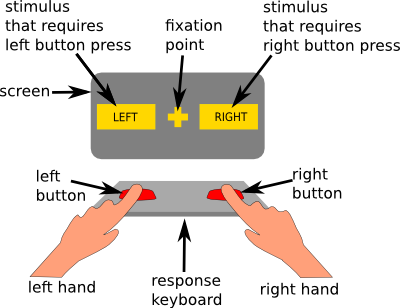
\includegraphics[width=0.5\textwidth]{13_Expyriment/simon.png}

    \note{

        \url{https://en.wikipedia.org/wiki/Simon_effect}

    }

\end{frame}

\begin{frame}[fragile]{Defining Constants}

    \begin{pythoncode}
from expyriment import design, control, stimuli, misc

POSITIONS = {
    "left": (-300, 0),
    "right": (300, 0),
}

COLORS = {
    "red": (255, 0, 0), 
    "green": (0, 128, 0)
}
    \end{pythoncode}

    \note{

        These are only fragments of code for demonstration purposes.

        \vspace{1em}

        You can find the full code in the file \texttt{simon.py} on StudIP.

    }

\end{frame}


\begin{frame}[fragile]{Defining Constants}

    \begin{pythoncode}
KEY_MAPPING = {
    misc.constants.K_s: "left", 
    misc.constants.K_l: "right"
}

PAIRINGS = {
    "red_left_green_right": ("s", "l"),
    "red_right_green_left": ("l", "s")
}
    \end{pythoncode}

    \note{

        These are only fragments of code for demonstration purposes.

        \vspace{1em}

        You can find the full code in the file \texttt{simon.py} on StudIP.

    }

\end{frame}


\begin{frame}[fragile]{Performing the Experiment}

    \begin{pythoncode}
def perform_simon_task():
    """Performs a Simon Task experiment."""

    exp = design.Experiment("Simon Task")
    control.initialize(exp)
    
    exp = design_experiment(exp, [...])

    exp.data_variable_names = ["position", [...]]

    control.start()
    execute_experiment(exp, [...])
    control.end()
    \end{pythoncode}

    \note{

        These are only fragments of code for demonstration purposes.

        \vspace{1em}

        You can find the full code in the file \texttt{simon.py} on StudIP.

    }

\end{frame}


\begin{frame}[fragile]{Designing the Experiment}

    \begin{pythoncode}
def design_experiment(exp, positions, colors, pairings):
    """Designs a Simon Task experiment."""

    for pair_name, pairing in pairings.items():
        
        b = design.Block()
        b.set_factor("pairing", pair_name) 

    \end{pythoncode}

    \note{

        These are only fragments of code for demonstration purposes.

        \vspace{1em}

        You can find the full code in the file \texttt{simon.py} on StudIP.

    }

\end{frame}


\begin{frame}[fragile]{Designing the Experiment}

    \begin{pythoncode}
for pos_name, position in positions.items():
    for color_name, color in colors.items():

        t = design.Trial()
        t.set_factor("position", pos_name)
        t.set_factor("color", color_name)
        s = stimuli.Rectangle((50, 50), [...])
        t.add_stimulus(s)
        b.add_trial(t, copies=20)

b.shuffle_trials()
exp.add_block(b)

    \end{pythoncode}

    \note{

        These are only fragments of code for demonstration purposes.

        \vspace{1em}

        You can find the full code in the file \texttt{simon.py} on StudIP.

    }

\end{frame}


\begin{frame}[fragile]{Executing the Experiment}

    \begin{pythoncode}
def execute_experiment(exp, text, key_mapping, pairings):
    """Executes a predesigned Simon Task experiment."""

    fixcross = stimuli.FixCross()
    fixcross.preload()

    for block in exp.blocks:

        pairing = pairings[block.get_factor("pairing")]
        instructions = text.format(*pairing)

        stimuli.TextScreen([...], instructions).present()
        exp.keyboard.wait()
    \end{pythoncode}

\end{frame}

\begin{frame}[fragile]{Executing the Experiment}

    \begin{pythoncode}
for trial in block.trials:

    fixcross.present()

    exp.clock.wait(1000 - trial.stimuli[0].preload())
    trial.stimuli[0].present()

    key, rt = exp.keyboard.wait(keys=key_mapping.keys())

    exp.data.add([block.get_factor("position"), [...]])
    \end{pythoncode}

\end{frame}


\begin{frame}[fragile]{After the Experiment}

    During the experiment, two folders are created: \textbf{data} and \textbf{events}.

    \vspace{1em}

    \textbf{data} contains one file for each subject in which the values of the predefined variables are stored for each trial .
    
    \vspace{1em}

    \textbf{events} contains one file for each subject in which a detailed stimulus-response protocol is stored.

    \vspace{1em}

    The files end on \texttt{.xpd} (\textit{expyriment data}) and \texttt{.xpe} (\textit{expyriment event}), but they can be opened just like the CSV files that we already know.

\end{frame}


\section{Organisational}


\begin{frame}[plain]
    \sectionpage
\end{frame}


\begin{frame}[fragile]{Passing the Course}

    To pass this course, you need 10 homework points. Each sheet you passed gives you 1 homework point.

    \vspace{1em}

    To pass a sheet, you need at least 60 percent of the points.

    \vspace{1em}

    \textbf{Good News:} Most of you already have 10 points (you should have gotten a mail by now).

    \vspace{1em}

    If you were not able to get 10 homework points from the sheets alone, you will have to do a project if you want to pass the course.

    \vspace{1em}

    \textbf{The deadline for project proposals is 14.07.2019}.

    \note{

        You can reach us here:

        \begin{itemize}

            \item mpoemsl@uos.de
            \item kgross@uos.de
            \item sselbach@uos.de
        
        \end{itemize}

    }


\end{frame}


\begin{frame}[fragile]{Topics You Now Know About}

    \begin{enumerate}

        \setcounter{enumi}{1}
        \item Variables and Assignments
        \item Control Structures
        \item Data Structures
        \item Strings
        \item Input and Output
        \item Good Practices
        \item Standard Library
        \item Object-Oriented Programming
        \item Recap
        \item Pythonic Programming
        \item Webscraping
        \item Expyriment

    \end{enumerate}

\end{frame}


\begin{frame}[fragile]{What's next?}

    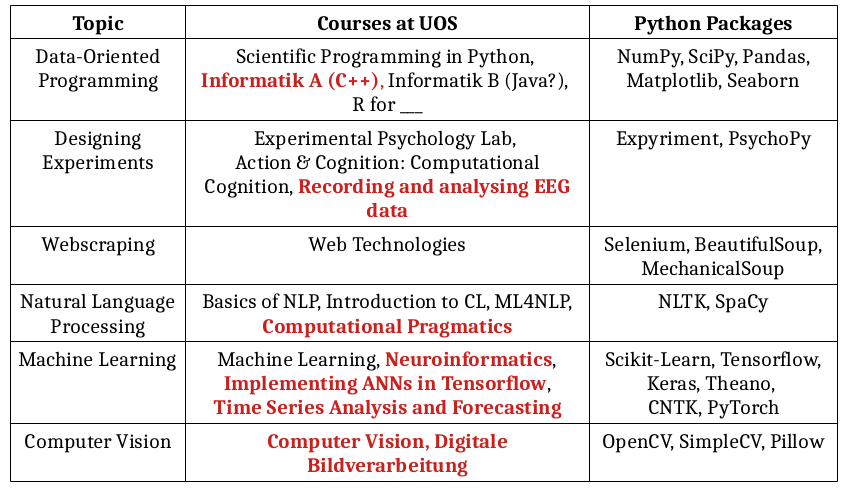
\includegraphics[width=\textwidth]{13_Expyriment/table.png}

    \note{

        The courses marked in red are the ones that will definitely be offered in the next semester (WS 2019/20).

        \vspace{1em}

        Those not marked in red may also be offered, but are not announced yet.

    }

\end{frame}


\begin{frame}{Evaluation}

    I know this is the third time you are asked to do this, but \textbf{please use the TAN you just received to evaluate me.}

    \vspace{1em}

    \centering 
\includegraphics[width=0.5\textwidth]{13_Expyriment/jules.jpg}

    \vspace{1em}
    
    \textbf{This is the only feedback that I get.} No matter if you enjoyed the course or not, please let me know!

    \note{
    
        I enjoyed the lectures and practice sessions very much. 

    }

\end{frame}


\begin{frame}{Farewell}

    Thank you for your attention. Enjoy the summer break!

    \note{
    
        If there are any questions left, you can reach me here:

        \vspace{1em}

        \texttt{mpoemsl@uos.de}

    }

\end{frame}

\end{document}
